\documentclass{beamer}

\usepackage{graphicx}
\usepackage{textpos}
\usepackage{verbatim}
\usepackage{forest}
\usepackage{algorithm}
\usepackage{forest}
\usepackage[noend]{algpseudocode}
%\usepackage{algorithm2e}

\setbeamertemplate{caption}[numbered]

\usepackage{tikz}
\usetikzlibrary{shapes.geometric}
\usetikzlibrary{arrows,shapes,trees}
\usetikzlibrary{calc,shapes.multipart,chains,arrows}

\usepackage[dvipsnames]{xcolor}
\definecolor{pblue}{rgb}{0.13,0.13,1}
\definecolor{pgreen}{rgb}{0,0.5,0}
\definecolor{pred}{rgb}{0.9,0,0}
\definecolor{pgrey}{rgb}{0.46,0.45,0.48}

\usepackage{listings}
\lstset{language=Java,
    showspaces=false,
    showtabs=false,
    breaklines=true,
    showstringspaces=false,
    breakatwhitespace=true,
    commentstyle=\color{pgreen},
    keywordstyle=\color{pblue},
    stringstyle=\color{pred},
    basicstyle=\footnotesize,
    colframe=white!75!black,
    moredelim=[is][\textcolor{pgrey}]{\%\%}{\%\%}
}

\pgfdeclareshape{plain triangle}{
    \nodeparts{}
    \anchor{center}{\pgfpoint{0cm}{0cm}}
    \behindbackgroundpath{
        \path [draw,dashed] (0,0) -- (.5,-1) -- (-0.5,-1) -- cycle;
    }
    \pgfsetcolor{red}
}

\pgfdeclareshape{blue triangle}{
    \nodeparts{}
    \anchor{center}{\pgfpoint{0cm}{0cm}}
    \behindbackgroundpath{
        \path [draw,dashed, fill=blue] (0,0) -- (.5,-1) -- (-0.5,-1) -- cycle;
    }
    \pgfsetcolor{red}
}

\pgfdeclareshape{red triangle}{
    \nodeparts{}
    \anchor{center}{\pgfpoint{0cm}{0cm}}
    \behindbackgroundpath{
        \path [draw,dashed, fill=red] (0,0) -- (.5,-1) -- (-0.5,-1) -- cycle;
    }
    \pgfsetcolor{red}
}
\usetheme{Madrid}
\useoutertheme{miniframes} % Alternatively: miniframes, infolines, split



% Setup the university's color pallette
\definecolor{UIUCorange}{RGB}{19, 41, 75} % UBC Blue (primary)
\definecolor{UIUCblue}{RGB}{232, 74, 39} % UBC Grey (secondary)


\setbeamercolor{palette primary}{bg=UIUCorange,fg=white}
\setbeamercolor{palette secondary}{bg=UIUCblue,fg=white}
\setbeamercolor{palette tertiary}{bg=UIUCblue,fg=white}
\setbeamercolor{palette quaternary}{bg=UIUCblue,fg=white}
\setbeamercolor{structure}{fg=UIUCorange} % itemize, enumerate, etc
\setbeamercolor{section in toc}{fg=UIUCblue} % TOC sections

\setbeamercolor{subsection in head/foot}{bg=UIUCorange,fg=UIUCblue}
\setbeamercolor{subsection in head/foot}{bg=UIUCorange,fg=UIUCblue}

\usepackage[utf8]{inputenc}


%Information to be included in the title page:
\title{\textbf{AVL Trees}}
\author{\textbf{David H Smith IV}}
\institute[\textbf{UIUC}]{\textbf{University of Illinois Urbana-Champaign}}
\date{}

\setbeamertemplate{title page}[default][colsep=-4bp,rounded=true]
\addtobeamertemplate{title page}{\vspace{3\baselineskip}}{}
\addtobeamertemplate{title page}{
    \begin{textblock*}{\paperwidth}(-1.0em, -1.2em)
        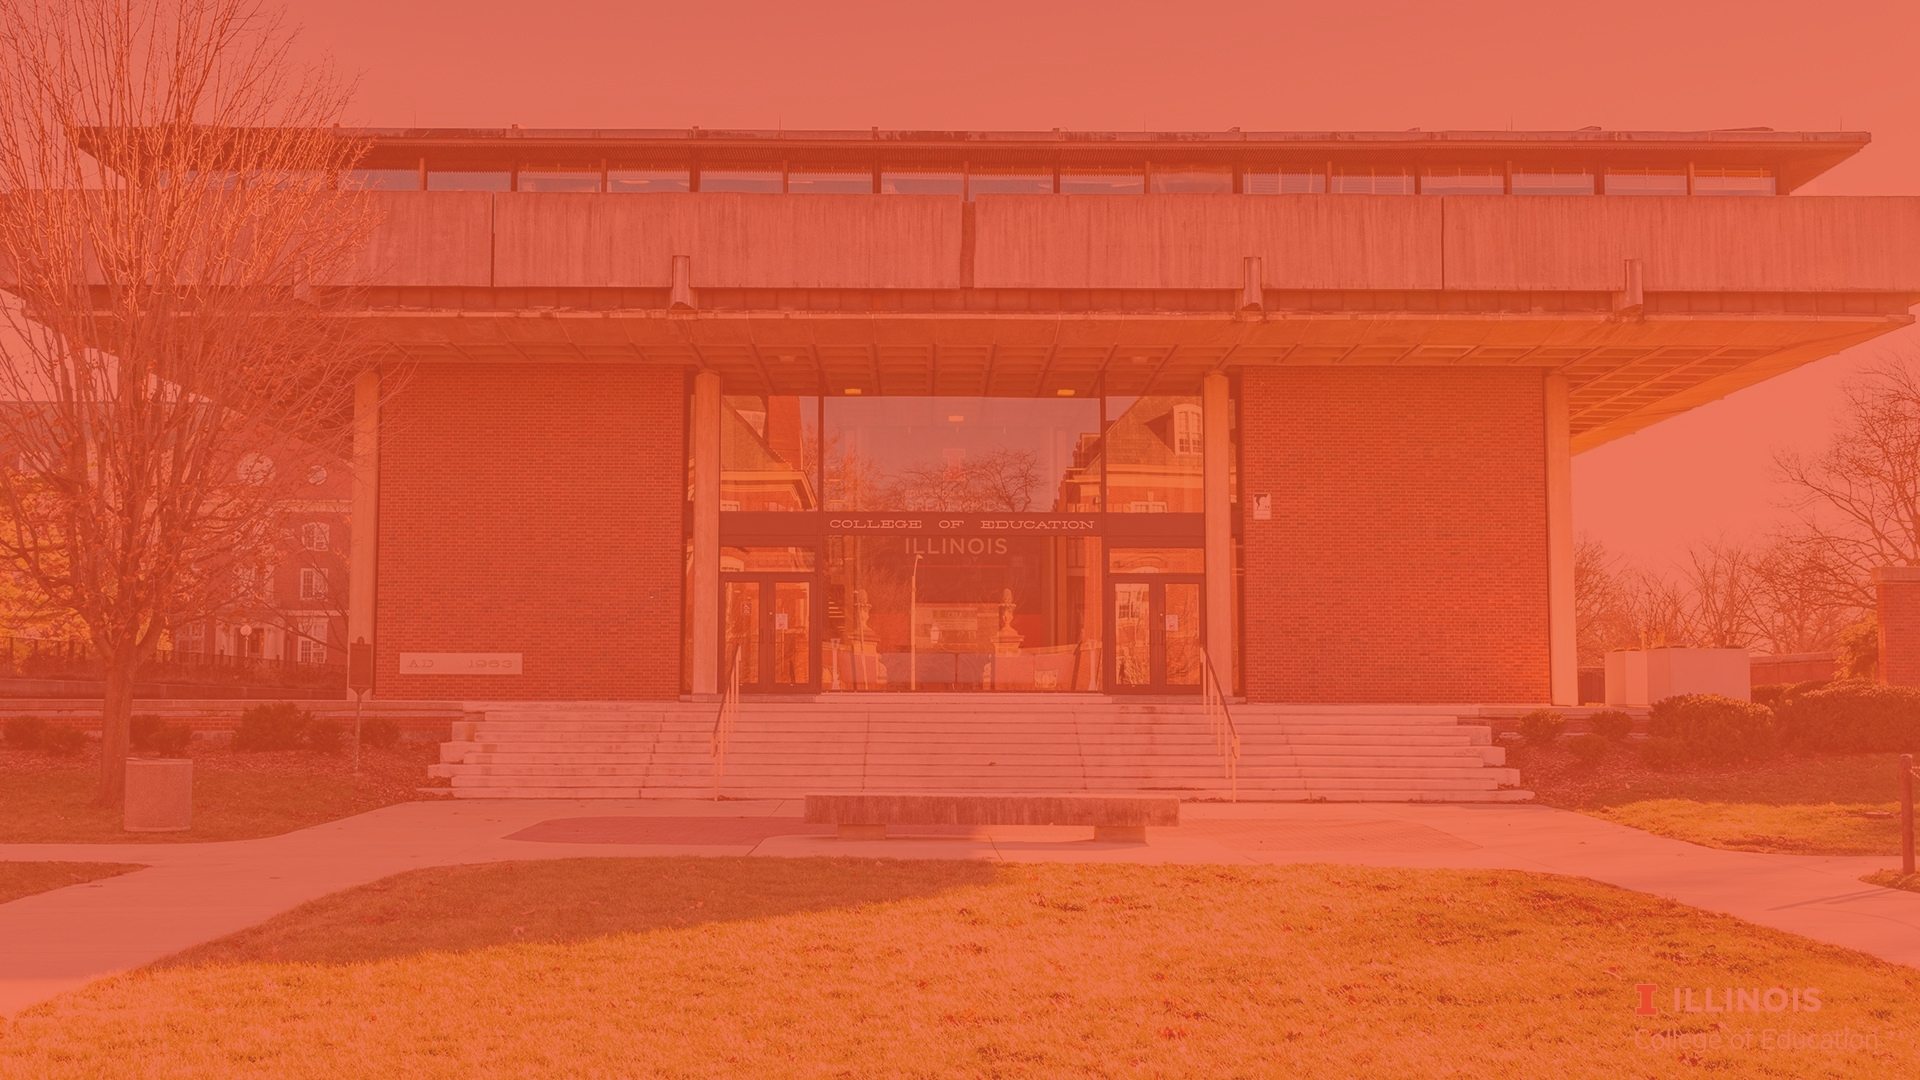
\includegraphics[width=\paperwidth, height=\paperheight]{imgs/uiuc.jpg}
    \end{textblock*} 
}{}

\begin{document}

\pgfdeclarelayer{background}
\pgfsetlayers{background,main}

\tikzstyle{vertex}=[circle,fill=black!25,minimum size=20pt,inner sep=0pt]
\tikzstyle{selected vertex} = [vertex, fill=orange!24]
\tikzstyle{edge} = [draw,thick,-]
\tikzstyle{weight} = [font=\small]
\tikzstyle{selected edge} = [draw,line width=5pt,-,blue!50]
\tikzstyle{ignored edge} = [draw,line width=5pt,-,black!20]


\frame{\titlepage}

\section{Objectives}
\begin{frame}
    \frametitle{Objectives}
    \centering
    \begin{itemize}
        \item Go over why we need to balance a BST in order to maintain $O(log_2(n))$ operations.
        \item Go over the relationship between height and balance factor.
        \item Cover how balance factor is used to determine what rotation to perform, if any, during recursive unwrapping.
        \item Cover the four rotations: right, left, right-left, left-right. 
        \item \textbf{Assignment:} Transform a standard BST class into an AVL class.
    \end{itemize}
\end{frame}

\section{Why Balance}
\begin{frame}[fragile]
    \frametitle{BST Insert: A Nice Insertion Order}
    \begin{minipage}{0.45\textwidth}
        \begin{figure}
            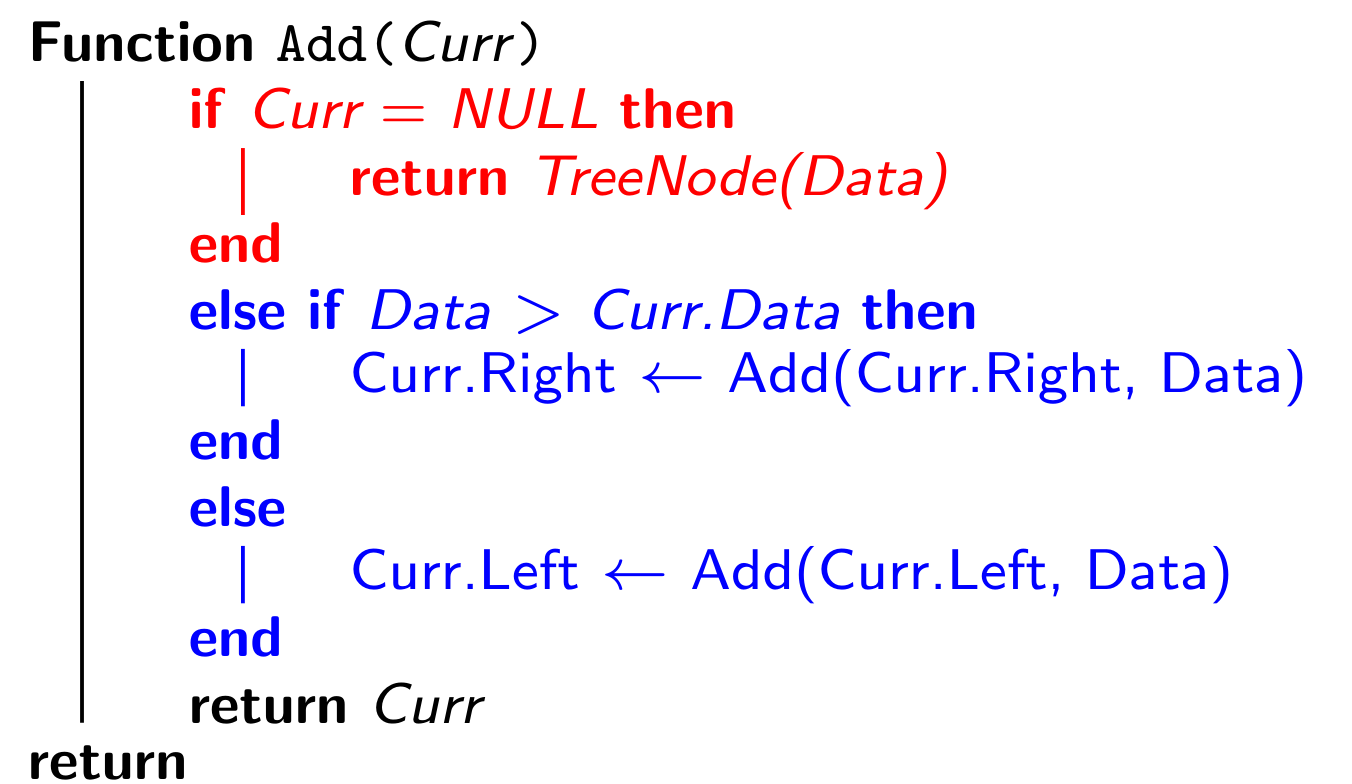
\includegraphics[width=\textwidth]{./imgs/bstadd.png}
        \end{figure}
        \begin{lstlisting}[frame=trBL, basicstyle=\tiny]
BST<Integer> bst = new BST<>();
bst.add(5)
bst.add(3)
bst.add(7)
bst.add(1)
bst.add(4)
bst.add(6)
bst.add(8)
        \end{lstlisting}
    \end{minipage}
    \begin{minipage}{0.45\textwidth}
    \end{minipage}
    \pause 
    \\\textbf{Time Complexity: } $O(log_{2}(n))$
\end{frame}

\begin{frame}[fragile]
    \frametitle{BST Insert: A Not-So-Nice Insertion Order}
    \begin{minipage}{0.45\textwidth}
        \begin{figure}
            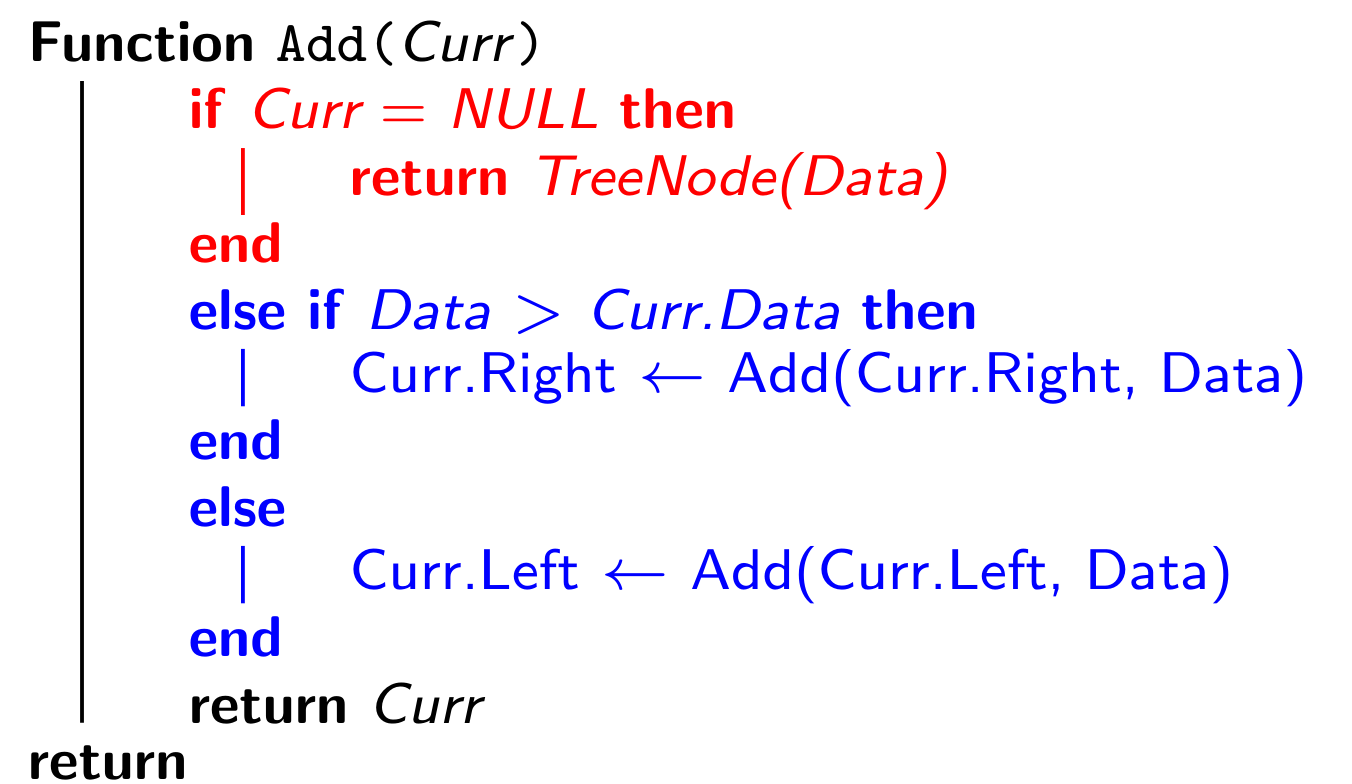
\includegraphics[width=\textwidth]{./imgs/bstadd.png}
        \end{figure}
        \begin{lstlisting}[frame=trBL, basicstyle=\tiny]
BST<Integer> bst = new BST<>();
bst.add(8)
bst.add(7)
bst.add(6)
bst.add(5)
bst.add(4)
bst.add(3)
bst.add(1)
        \end{lstlisting}
    \end{minipage}
    \begin{minipage}{0.45\textwidth}
    \end{minipage}
    \pause 
    \\\textbf{Time Complexity: } $O(n)$, Back at linked lists!
\end{frame}

\begin{frame}
    \frametitle{Goal: Avoid $O(n)$ Search Trees}

    \begin{minipage}{0.49\textwidth}
        \resizebox{!}{\textwidth}{
        \begin{forest}
            for tree={
                circle,
                black,
                draw
            }
            [{0}, edge label={node [midway, above left] {}}
            [,phantom]
            [{1}, edge label={node [midway, right] {}}
            [,phantom]
            [{2}, edge label={node [midway, right] {}}
            [,phantom]
            [{3}, edge label={node [midway, left] {}}
            [,phantom]
            [{4}, edge label={node [midway, left] {}}, 
            [,phantom]
            [{...}, edge label={node [midway, left] {}}, 
            [,phantom]
            [{12}, edge label={node [midway, left] {}}, 
            [,phantom]
            [{13}, edge label={node [midway, left] {}}, 
            [,phantom]
            [{14}, edge label={node [midway, left] {}}, 
            ]
            ]
            ]
            ]
            ]
            ]
            ]
            ]
            ]
        \end{forest}}
    \end{minipage}
    \begin{minipage}{0.49\textwidth}
        \resizebox{!}{0.49\textwidth}{
        \begin{forest}
            for tree={
                circle,
                black,
                draw
            }
            [{7}, edge label={node [midway, above right] {}}
            [{3}, edge label={node [midway, above left] {}}
            [{1}, edge label={node [midway, above left] {}}
            [{0}, edge label={node [midway, above left] {}}
            ],
            [{2}, edge label={node [midway, above left] {}}
            ]
            ],
            [{5}, edge label={node [midway, above left] {}}
            [{4}, edge label={node [midway, above left] {}}
            ],
            [{6}, edge label={node [midway, above left] {}}
            ]
            ]
            ]
            [{11}, edge label={node [midway, above right] {}}
            [{9}, edge label={node [midway, above left] {}}
            [{8}, edge label={node [midway, above left] {}}
            ],
            [{10}, edge label={node [midway, above left] {}}
            ]
            ],
            [{13}, edge label={node [midway, above left] {}}
            [{12}, edge label={node [midway, above left] {}}
            ],
            [{14}, edge label={node [midway, above left] {}}
            ]
            ]
            ]
            ]
        \end{forest}}
    \end{minipage}
    \\We want to ensure that we get the tree on the right \textit{regardless of the order in which we insert the nodes.}
\end{frame}


\section{AVL vs BST Nodes}
\begin{frame}[fragile]
    \frametitle{Comparing TreeNodes: AVL vs Standard BST}
    \begin{minipage}{0.45\textwidth}
        \textbf{Standard BST TreeNode}
        \begin{lstlisting}[frame=trBL]
static class TreeNode<E>{

    E data;
    TreeNode<E> left;
    TreeNode<E> right;

    TreeNode(data){
        this.data = data;
        left = null;
        right = null;
    }
}
        \end{lstlisting}
    \end{minipage}
    \hfill
    \begin{minipage}{0.45\textwidth}
        \textbf{AVL TreeNode}
        \begin{lstlisting}[frame=trBL]
static class TreeNode<E>{

    E data;
    int height;
    TreeNode<E> left;
    TreeNode<E> right;

    TreeNode(data){
        this.data = data;
        height = 0;
        left = null;
        right = null;
    }
}
        \end{lstlisting}
    \end{minipage}
    \vfill
    \textbf{TreeNode for AVL adds a height attribute!}
    \vfill
\end{frame}


\section{Insertion + Height}

\begin{frame}[fragile]
    \frametitle{How we got here!}

    \begin{minipage}{0.49\textwidth}
        \centering
        \begin{figure}
            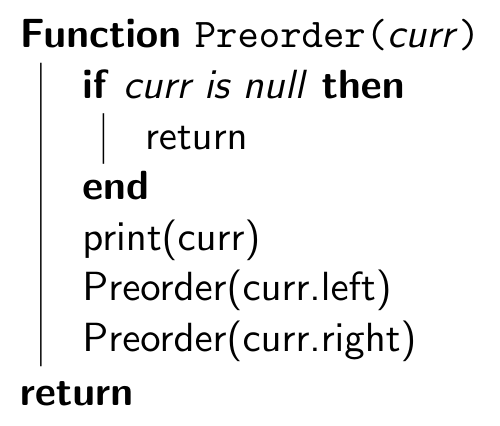
\includegraphics[width=0.49\textwidth]{./imgs/preorder.png}
            \caption{\scriptsize Binary Tree Traversal}
        \end{figure}
        \vspace{-0.5cm}
    \end{minipage}
    \vline
    \begin{minipage}{0.49\textwidth}
        \centering
        \begin{figure}
            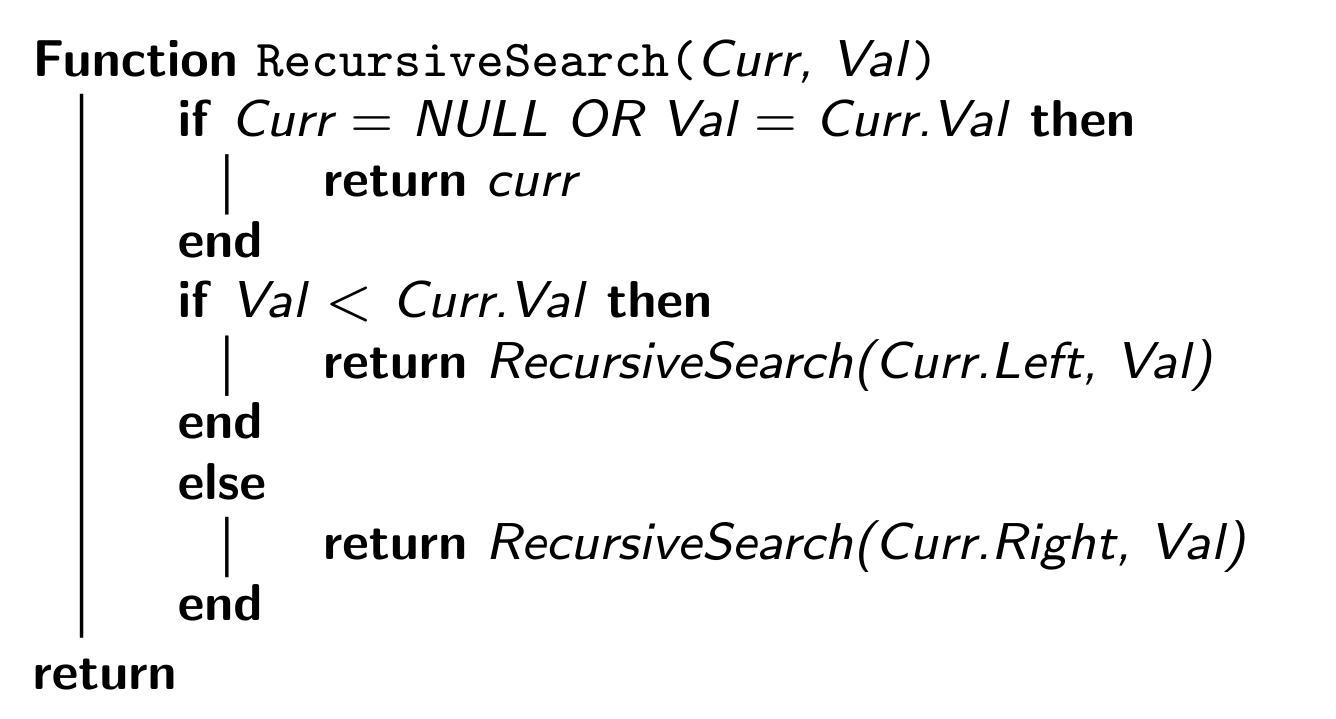
\includegraphics[width=0.79\textwidth]{./imgs/bstsearch.png}
            \caption{\scriptsize BST Search}
        \end{figure}
    \end{minipage}
    \\
    \hline
    \\
    \begin{minipage}{0.49\textwidth}
        \centering
        \begin{figure}
            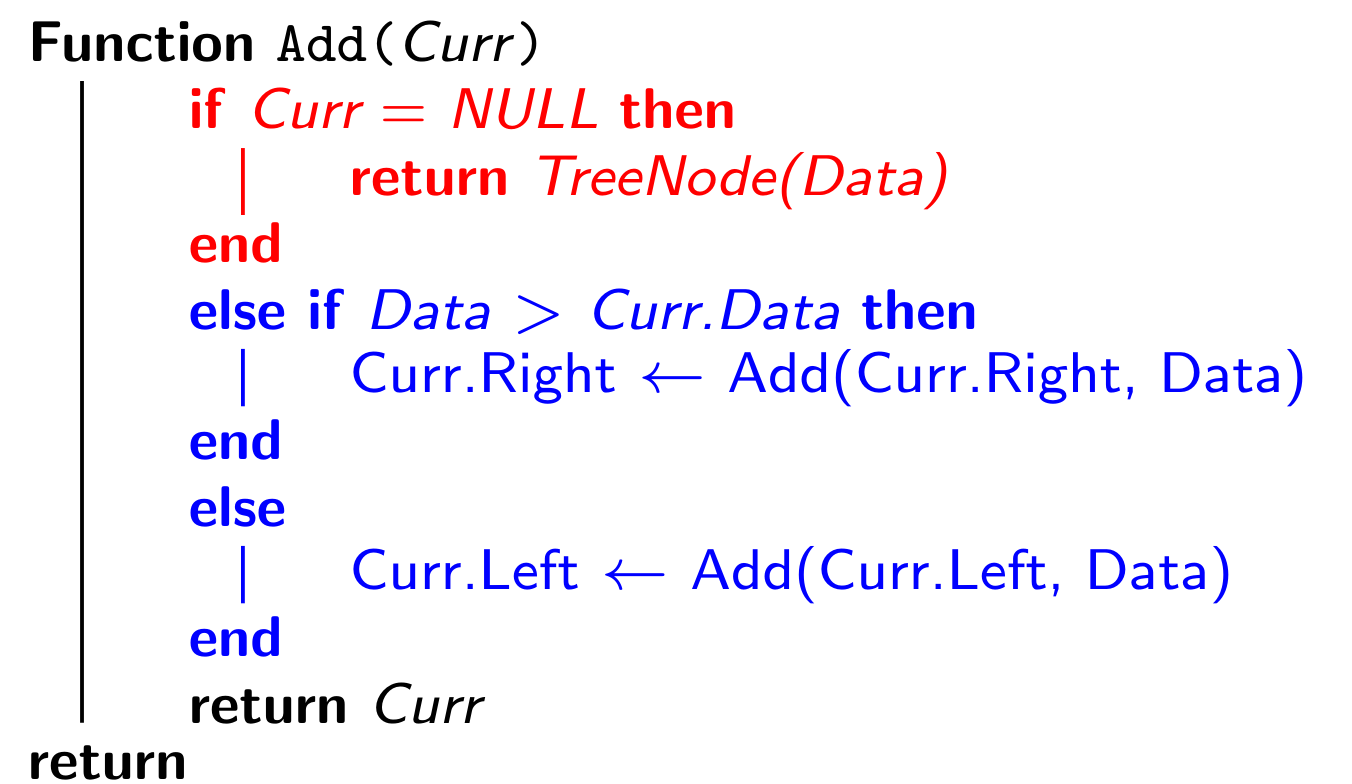
\includegraphics[width=0.75\textwidth]{./imgs/bstadd.png}
            \caption{\scriptsize BST Add}
        \end{figure}
    \end{minipage}
    \vline
    \begin{minipage}{0.49\textwidth}
        \centering
        \begin{figure}
            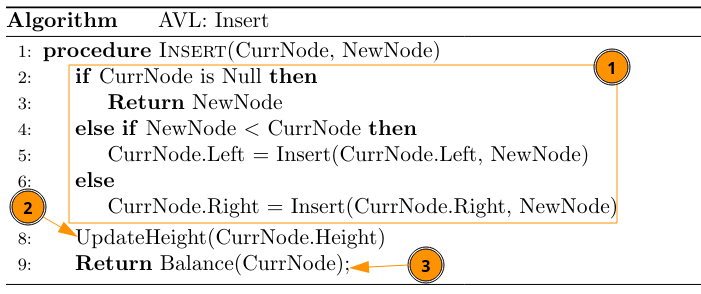
\includegraphics[width=\textwidth]{./imgs/avl-insert-annotate-algo.png}
            \caption{\scriptsize AVL Tree Add}
        \end{figure}
    \end{minipage}
\end{frame}

\begin{frame}[fragile]
    \frametitle{AVL Insertion}
    \begin{figure}
        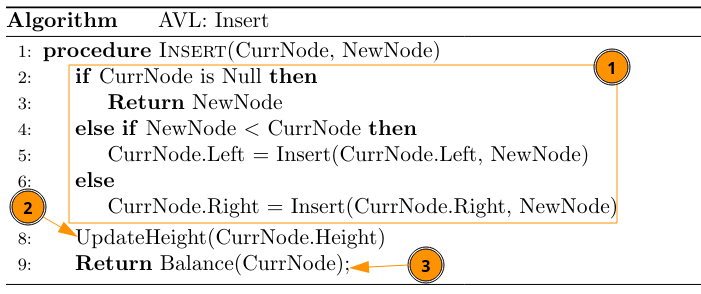
\includegraphics[width=0.7\textwidth]{./imgs/avl-insert-annotate-algo.png}
    \end{figure}
    \begin{enumerate}
        \item Block (1) is \textit{identical} to BST insert
        \item The main difference between BST and AVL is in the recursive unwrap.
        \begin{enumerate}
            \item Before returning (2) we need to update the height of each node that we traversed over.
            \item We also need to ensure that everything is balanced (3) with respect to that node.
        \end{enumerate}
    \end{enumerate}
\end{frame}

\begin{frame}[fragile]
    \frametitle{Lets Take a Look at Height First}
    \begin{minipage}{0.24\textwidth}
        \begin{lstlisting}[frame=trBL, basicstyle=\small]
bst.add(5)
bst.add(3)
bst.add(7)
bst.add(1)
bst.add(4)
bst.add(6)
bst.add(8)
        \end{lstlisting}
    \end{minipage}
    \begin{minipage}{0.74\textwidth}
        \hfill
    \end{minipage}
    \vfill
    \textbf{Update Height Equation:} $Node.Height = Max(Node.Left.Height, Node.Right.Height) + 1$
\end{frame}


\section{Balance Factor}
\begin{frame}
    \frametitle{Balance Factor}
    \begin{enumerate}
        \item \textbf{Balance Factor Equation:} $BF = Node.Left.Height - Node.Right.Height$
        \item We use the balance factor equation to determine:
            \begin{enumerate}
                \item When we need to rotate
                \item What type of rotation needs to be performed.
            \end{enuemrate}
        \item \textit{Important!} If \texttt{left} or \texttt{right} are \lstinline|null| we treat their height as $-1$.
    \end{enumerate}
\end{frame}

\section{Balancing Subtrees}
\begin{frame}[fragile]
    \frametitle{AVL Balance Method: Right Rotations}
    \begin{minipage}{0.44\textwidth}
        \begin{algorithm}[H]
            \caption{AVL: Balance}
            \scriptsize
            \begin{algorithmic}[1]
                \Procedure{Balance}{N}
                \color{red}
                \If{BF(N) $>$ 1}
                \If{BF(N.left) $<$ 0}
                \State N = RotateLeftRight(N)
                \Else
                \State N = Right(N)
                \EndIf
                \color{black}
                \ElsIf{BF(N) $<$ -1}
                \If{BF(N.right) $>$ 0}
                \State N = RotateRightLeft(N)
                \Else
                \State N = Left(N)
                \EndIf
                \EndIf
                \State \textbf{Return} N
                \EndProcedure
            \end{algorithmic}
        \end{algorithm}
    \end{minipage}
    \hfill
    \begin{minipage}{0.44\textwidth}
    \end{minipage}
    \vfill
    \\Unbalanced with respect to left subtree (BF $>$ 1).
    \vfill

    \end{frame}
\begin{frame}[fragile]
    \frametitle{AVL Balance Method: Right Rotations}
    \begin{minipage}{0.44\textwidth}
        \begin{algorithm}[H]
            \caption{AVL: Balance}
            \scriptsize
            \begin{algorithmic}[1]
                \Procedure{Balance}{N}
                \If{BF(N) $>$ 1}
                \color{orange}
                \If{BF(N.left) $<$ 0}
                \State N = RotateLeftRight(N)
                \color{blue}
                \Else
                \State N = Right(N)
                \EndIf
                \color{black}
                \ElsIf{BF(N) $<$ -1}
                \If{BF(N.right) $>$ 0}
                \State N = RotateRightLeft(N)
                \Else
                \State N = Left(N)
                \EndIf
                \EndIf
                \State \textbf{Return} N
                \EndProcedure
            \end{algorithmic}
        \end{algorithm}
    \end{minipage}
    \hfill
    \begin{minipage}{0.44\textwidth}
    \end{minipage}
    \end{frame}

\begin{frame}[fragile]
    \frametitle{AVL Balance Method: Left Rotations}
    \begin{minipage}{0.44\textwidth}
        \begin{algorithm}[H]
            \caption{AVL: Balance}
            \scriptsize
            \begin{algorithmic}[1]
                \Procedure{Balance}{N}
                \If{BF(N) $>$ 1}
                \If{BF(N.left) $<$ 0}
                \State N = RotateLeftRight(N)
                \Else
                \State N = Right(N)
                \EndIf
                \color{red}
                \ElsIf{BF(N) $<$ -1}
                \If{BF(N.right) $>$ 0}
                \State N = RotateRightLeft(N)
                \Else
                \State N = Left(N)
                \EndIf
                \EndIf
                \color{black}
                \State \textbf{Return} N
                \EndProcedure
            \end{algorithmic}
        \end{algorithm}
    \end{minipage}
    \begin{minipage}{0.24\textwidth}
    \end{minipage}
    \vfill
    \\Unbalanced with respect to right subtree (BF $<$ -1).
    \vfill
\end{frame}

\begin{frame}[fragile]
    \frametitle{AVL Balance Method: Left Rotations}
    \begin{minipage}{0.44\textwidth}
        \begin{algorithm}[H]
            \caption{AVL: Balance}
            \scriptsize
            \begin{algorithmic}[1]
                \Procedure{Balance}{N}
                \If{BF(N) $>$ 1}
                \If{BF(N.left) $<$ 0}
                \State N = RotateLeftRight(N)
                \Else
                \State N = Right(N)
                \EndIf
                \ElsIf{BF(N) $<$ -1}
                \color{orange}
                \If{BF(N.right) $>$ 0}
                \State N = RotateRightLeft(N)
                \color{blue}
                \Else
                \State N = Left(N)
                \EndIf
                \EndIf
                \color{black}
                \State \textbf{Return} N
                \EndProcedure
            \end{algorithmic}
        \end{algorithm}
    \end{minipage}
    \begin{minipage}{0.24\textwidth}
    \end{minipage}
\end{frame}

\section{Rotations}
\begin{frame}
    \frametitle{Right Rotation}
    \begin{minipage}{0.49\textwidth}
    \begin{algorithm}[H]
        \caption{AVL: Right Rotation}\label{}
        \begin{algorithmic}[1]
            \Procedure{Right}{N}
            \State Tmp = N.Left
            \State N.Left = Tmp.Right;
            \State Tmp.Right = N
            \State 
            \State UpdateHeight(N)
            \State UpdateHeight(Tmp)
            \State
            \State \textbf{Return} Tmp
            \EndProcedure
        \end{algorithmic}
    \end{algorithm}
    \end{minipage}
    \begin{minipage}{0.49\textwidth}
        \hfill
    \end{minipage}
\end{frame}

\begin{frame}
    \frametitle{Left Rotation}
    \begin{minipage}{0.49\textwidth}
    \begin{algorithm}[H]
        \caption{AVL: Left Rotation}\label{}
        \begin{algorithmic}[1]
            \Procedure{Left}{N}
            \State Tmp = N.Right
            \State N.Right = Tmp.Left;
            \State Tmp.Left = N
            \State 
            \State UpdateHeight(N)
            \State UpdateHeight(Tmp)
            \State
            \State \textbf{Return} Tmp
            \EndProcedure
        \end{algorithmic}
    \end{algorithm}
    \end{minipage}
    \begin{minipage}{0.49\textwidth}
        \hfill
    \end{minipage}
\end{frame}

\begin{frame}
    \frametitle{Left-Right Rotation}
    \vspace{4cm}
    \begin{algorithm}[H]
        \caption{AVL: LeftRightRotate}\label{}
        \begin{algorithmic}[1]
            \Procedure{LeftRightRotate}{N}
            \State N.Left = Left(N.Left)
            \State \textbf{Return} Right(N)
            \EndProcedure
        \end{algorithmic}
    \end{algorithm}
\end{frame}

\begin{frame}
    \frametitle{Right-Left Rotation}
    \vspace{4cm}
    \begin{algorithm}[H]
        \caption{AVL: RightLeftRotate}\label{}
        \begin{algorithmic}[1]
            \Procedure{RightLeftRotate}{N}
            \State N.Right = Right(N.Right)
            \State \textbf{Return} Left(N)
            \EndProcedure
        \end{algorithmic}
    \end{algorithm}
\end{frame}

\begin{frame}[fragile]
    \frametitle{Putting it all together\ldots}
    \begin{minipage}{0.49\textwidth}
        \begin{algorithm}[H]
            \caption{AVL: Balance}
            \tiny
            \begin{algorithmic}[1]
                \Procedure{Balance}{N}
                \If{BF(N) $>$ 1}
                \If{BF(N.left) $<$ 0}
                \State N = RotateLeftRight(N)
                \Else
                \State N = Right(N)
                \EndIf
                \ElsIf{BF(N) $<$ -1}
                \If{BF(N.right) $>$ 0}
                \State N = RotateRightLeft(N)
                \Else
                \State N = Left(N)
                \EndIf
                \EndIf
                \State \textbf{Return} N
                \EndProcedure
            \end{algorithmic}
        \end{algorithm}
        \begin{lstlisting}[frame=trBL, basicstyle=\tiny]
bst.add(8)
bst.add(7)
bst.add(6)
bst.add(5)
bst.add(4)
bst.add(3)
bst.add(1)
        \end{lstlisting}
    \end{minipage}
    \begin{minipage}{0.49\textwidth}
        \hfill
    \end{minipage}
\end{frame}



\section{Remove}
\begin{frame}
    \frametitle{AVL Remove: It's the same changes as Add!}
    \vfill
    \begin{figure}
        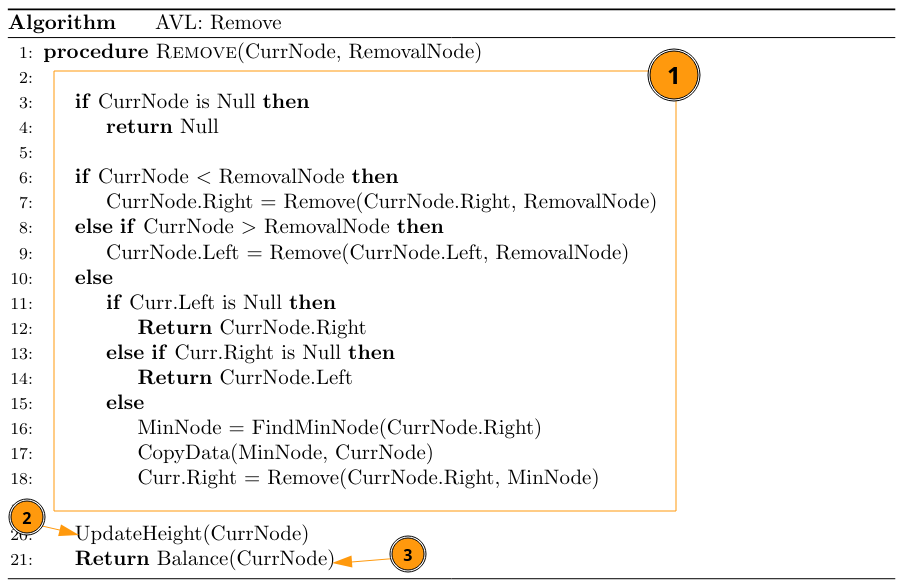
\includegraphics[width=0.75\textwidth]{./imgs/avl-remove-algo-annotated.png}
    \end{figure}
    \vfill
\end{frame}




\end{document}
